%%
% This is an Overleaf template for presentations
% using the TUM Corporate Desing https://www.tum.de/cd
%
% For further details on how to use the template, take a look at our
% GitLab repository and browse through our test documents
% https://gitlab.lrz.de/latex4ei/tum-templates.
% The tumbeamer class is based on the beamer class.
% If you need further customization please consult the beamer class guide
% https://ctan.org/pkg/beamer.
% Additional class options are passed down to the base class.
%
% If you encounter any bugs or undesired behaviour, please raise an issue
% in our GitLab repository
% https://gitlab.lrz.de/latex4ei/tum-templates/issues
% and provide a description and minimal working example of your problem.
%%


\documentclass[
  english,            % define the document language (english, german)
  aspectratio=169,    % define the aspect ratio (169, 43)
  % handout=2on1,       % create handout with multiple slides (2on1, 4on1)
  % partpage=false,     % insert page at beginning of parts (true, false)
  % sectionpage=true,   % insert page at beginning of sections (true, false)
]{tumbeamer}


% load additional packages
\usepackage{booktabs}

\usepackage[utf8]{inputenc}
\usepackage{xcolor}
\usepackage{tikz}
\usetikzlibrary{calc}
\usetikzlibrary{arrows.meta}
\usetikzlibrary{positioning}
\usepackage{amsmath}
\usepackage{amsfonts}
%\usepackage{todonotes}
\newcommand\todo[1]{\textit{\textcolor{blue}{\\TODO: #1\\}}}
\newcommand\todoi[1]{\textit{\textcolor{blue}{TODO: #1}}}
\newcommand\tcb[1]{\textit{\textcolor{blue}{#1}}}

\newcommand\bx[0]{\textbf{x}}
\newcommand\by[0]{\textbf{y}}
\newcommand\bomega[0]{\boldsymbol{\omega}}

\usepackage{mathtools}

\newcommand*\mystrut[1]{\vrule width0pt height0pt depth#1\relax}

\usepackage{import}
\usepackage{xifthen}
\usepackage{pdfpages}
\usepackage{transparent}
\newcommand{\incfig}[1]{%
    \def\svgwidth{\columnwidth}
    \import{./img/}{#1.pdf_tex}
}

\usepackage{bm}

% presentation metadata
\title{Rendering Participating Media}
\subtitle{Data Visualization Seminar}
\author{Barnabás Börcsök}

\institute{\theChairName\\\theDepartmentName\\\theUniversityName}
\date[WS 2021/2022]{Winter Semester, 2021/2022}

\footline{\insertauthor~|~\insertshorttitle~|~\insertshortdate}


% macro to configure the style of the presentation
\TUMbeamersetup{
  title page = TUM centered,         % style of the title page
  part page = TUM toc,            % style of part pages
  section page = TUM toc,         % style of section pages
  content page = TUM more space,  % style of normal content pages
  tower scale = 1.0,              % scaling factor of TUM tower (if used)
  headline = TUM threeliner,      % which variation of headline to use
  footline = TUM default,         % which variation of footline to use
  % configure on which pages headlines and footlines should be printed
  headline on = {title page},
  footline on = {every page, title page=false},
}

% available frame styles for title page, part page, and section page:
% TUM default, TUM tower, TUM centered,
% TUM blue default, TUM blue tower, TUM blue centered,
% TUM shaded default, TUM shaded tower, TUM shaded centered,
% TUM flags
%
% additional frame styles for part page and section page:
% TUM toc
%
% available frame styles for content pages:
% TUM default, TUM more space
%
% available headline options:
% TUM empty, TUM oneliner, TUM twoliner, TUM threeliner, TUM logothreeliner
%
% available footline options:
% TUM empty, TUM default, TUM infoline


\begin{document}

\maketitle

%\section{First Section}
\begin{frame}{Motivation}
  \begin{figure}
      \centering
      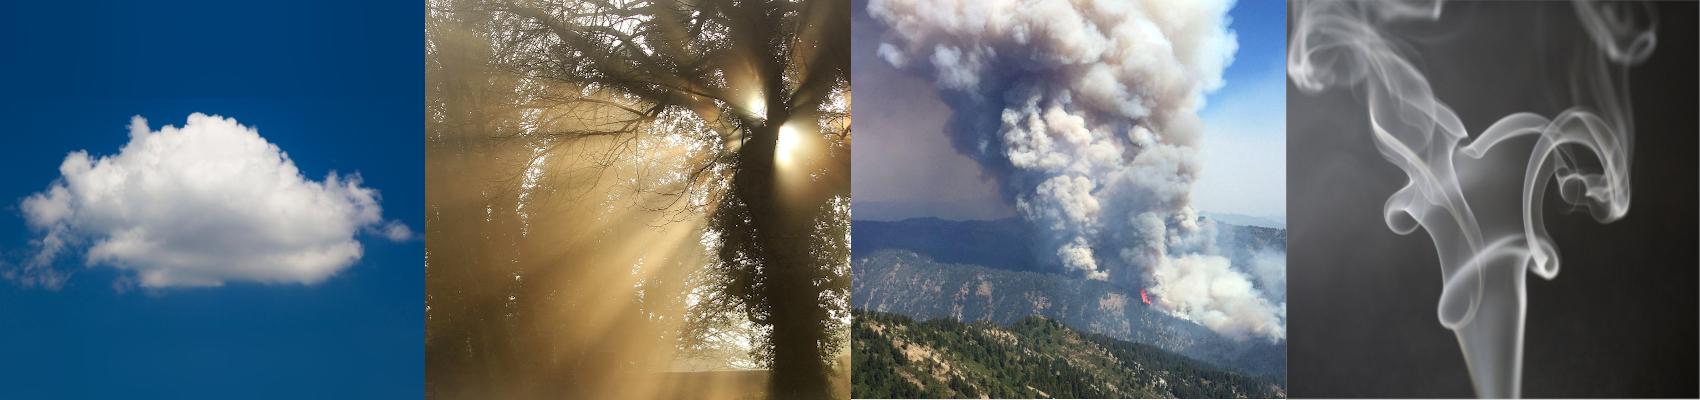
\includegraphics{img/teaser.png}
      \label{fig:teaser}
  \end{figure}
\end{frame}


\begin{frame}{Motivation}
  \begin{figure}
      \centering
      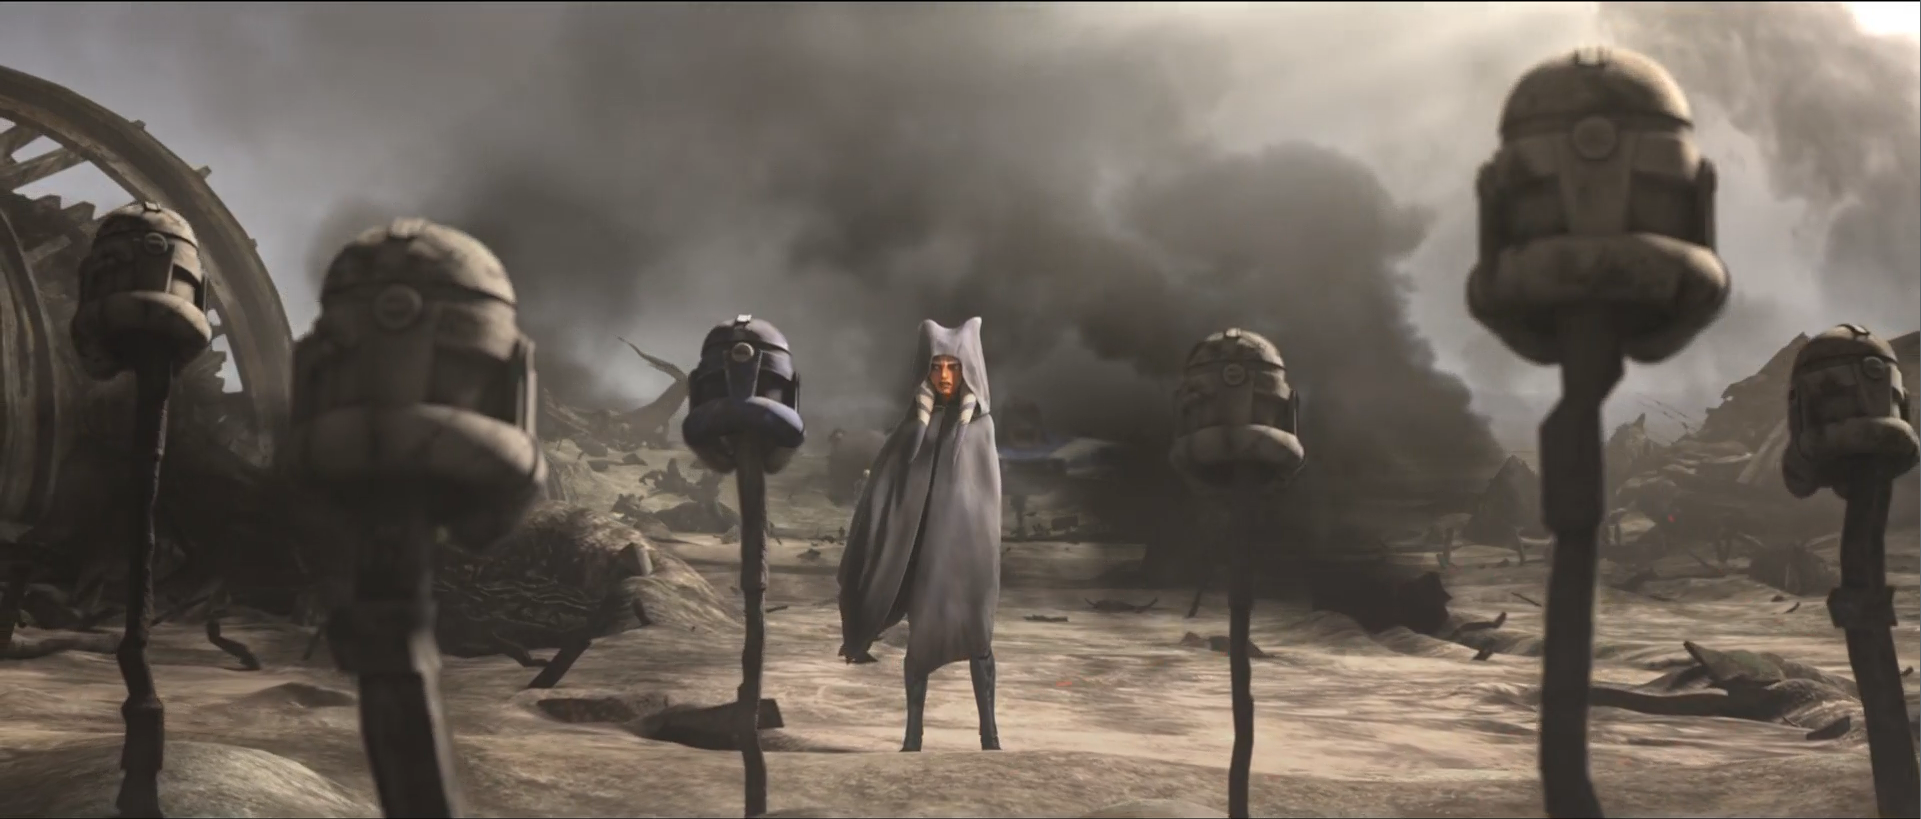
\includegraphics[width=\textwidth]{img/ahsoka-smoke.png}
      \label{fig:teaser}
  \end{figure}
\end{frame}

\begin{frame}{Propagation of light in a medium}
    \begin{figure}[ht]
        \centering
        \def\svgwidth{\columnwidth}
        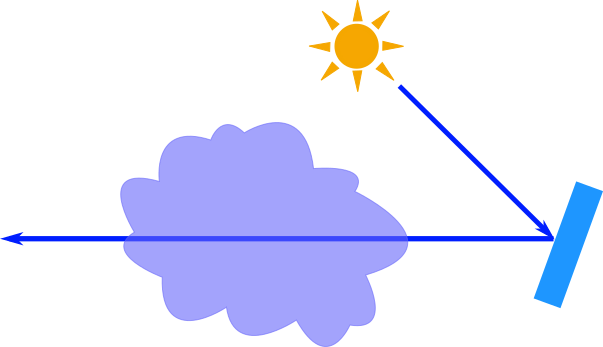
\includegraphics[width=10cm]{img/propagation-illustration.png}
        % \label{fig:propagation-illustration}
    \end{figure}
\end{frame}

\begin{frame}{Change of radiance in a differential volume}
    \begin{figure}[ht]
        \centering
        \incfig{differential_volume}
        \label{fig:vre}
    \end{figure}
\end{frame}


\begin{frame}{Possible interactions}{between the volume and the light
    traveling through the medium}
\begin{figure}[ht]
    \centering
    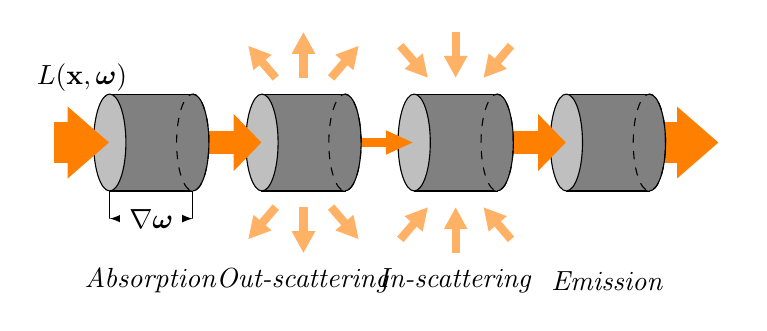
\begin{tikzpicture}
% 1 = 20p
    \def\XSTART{-10pt}
    \def\YSTART{60pt}
    \def\YDIAONE{35pt}
    \def\XONESTART{10pt}
    \def\XONEDELTA{30pt} %width of cylinders
    \def\DD{-10pt} %
    \def\GAP{25pt} %
    
    \def\LABELYSHIFT{-50pt}
    
    %FIRST cylinder
    \def\YEND{\YSTART+\YCURVE+\YDIATWO}
    \def\XONEEND{\XONESTART+\XONEDELTA}
    \def\YONEMIDDLE{\YSTART+\YDIAONE/2}
  
    %SECOND cylinder
    \def\XTWOSTART{\XONESTART+\XONEDELTA+\GAP}
    \def\XTWOEND{\XONEEND+\GAP+\XONEDELTA}
  
    %THIRD cylinder
    \def\XTHREESTART{\XONESTART+\XONEDELTA+\GAP+\XONEDELTA+\GAP}
    \def\XTHREEEND{\XONEEND+\GAP+\XONEDELTA+\GAP+\XONEDELTA}
    
    % FOURTH cylinder
    \def\XFOURSTART{\XONESTART+\XONEDELTA+\GAP+\XONEDELTA+\GAP+\XONEDELTA+\GAP}
    \def\XFOUREND{\XONEEND+\GAP+\XONEDELTA+\GAP+\XONEDELTA+\GAP+\XONEDELTA}

    \tikzset{
      partial ellipse/.style args={#1:#2:#3}{
          insert path={+ (#1:#3) arc (#1:#2:#3)}
      },
      dimen/.style={<->,>=latex,thin,
        every rectangle node/.style={fill=white,midway,font=\sffamily}},
    }
  
    % OUTGOING ARROW (EMISSION)
    \draw[-{Triangle[width=25pt,length=15pt, color=orange]}, 
            line width=15pt, color=orange]
        (\XFOUREND+0.5,\YONEMIDDLE) -- (\XFOUREND+\GAP,\YONEMIDDLE);

    %FOURTH CYLINDER
    \draw [fill=gray] (\XFOURSTART,\YSTART) coordinate (BA)
        rectangle (\XFOUREND,{\YSTART+\YDIAONE}) coordinate (BB);
    \draw [fill=lightgray](\XFOURSTART,\YONEMIDDLE)
        ellipse ({\YDIAONE/6} and {\YDIAONE/2});
    \draw [fill=gray,dashed](\XFOUREND,\YONEMIDDLE)
        ellipse ({\YDIAONE/6} and {\YDIAONE/2});
    \draw (\XFOUREND,\YONEMIDDLE)
        [partial ellipse=-90:90:{\YDIAONE/6} and {\YDIAONE/2}];

    \node[yshift=\LABELYSHIFT] at ($0.5*(BA)+0.5*(BB)$) {\textit{Emission}};

    % FIFTH ARROW (IN-SCATTERING)
    \draw[-{Triangle[width=20pt,length=10pt, color=orange]}, 
            line width=8pt, color=orange]
        (\XTHREEEND+0.5,\YONEMIDDLE) -- (\XTHREEEND+\GAP-0.2,\YONEMIDDLE);
    

    % INSCATTERING ARROWS AROUND THIRD CYLINDER
    % above
    \draw[-{Triangle[width=8pt,length=8pt, color=orange!60]}, 
            line width=3pt, color=orange!60]
        ({\XTHREESTART+\XONEDELTA/2},{\YONEMIDDLE+40pt}) --
        ({\XTHREESTART+\XONEDELTA/2},{\YONEMIDDLE+\YDIAONE/1.5});
    \draw[-{Triangle[width=8pt,length=8pt, color=orange!60]}, 
            line width=3pt, color=orange!60]
        ({\XTHREESTART+\XONEDELTA/2-20pt},{\YONEMIDDLE+35pt}) --
        ({\XTHREESTART+\XONEDELTA/2-10pt},{\YONEMIDDLE+\YDIAONE/1.5});
    \draw[-{Triangle[width=8pt,length=8pt, color=orange!60]}, 
            line width=3pt, color=orange!60]
        ({\XTHREESTART+\XONEDELTA/2+20pt},{\YONEMIDDLE+35pt}) --
        ({\XTHREESTART+\XONEDELTA/2+10pt},{\YONEMIDDLE+\YDIAONE/1.5});
    % below
    \draw[-{Triangle[width=8pt,length=8pt, color=orange!60]}, 
            line width=3pt, color=orange!60]
        ({\XTHREESTART+\XONEDELTA/2},{\YONEMIDDLE-40pt}) --
        ({\XTHREESTART+\XONEDELTA/2},{\YONEMIDDLE-\YDIAONE/1.5});
    \draw[-{Triangle[width=8pt,length=8pt, color=orange!60]}, 
            line width=3pt, color=orange!60]
        ({\XTHREESTART+\XONEDELTA/2-20pt},{\YONEMIDDLE-35pt}) -- 
        ({\XTHREESTART+\XONEDELTA/2-10pt},{\YONEMIDDLE-\YDIAONE/1.5});
    \draw[-{Triangle[width=8pt,length=8pt, color=orange!60]}, 
            line width=3pt, color=orange!60]
        ({\XTHREESTART+\XONEDELTA/2+20pt},{\YONEMIDDLE-35pt}) --
        ({\XTHREESTART+\XONEDELTA/2+10pt},{\YONEMIDDLE-\YDIAONE/1.5});

    \draw [fill=gray] (\XTHREESTART,\YSTART) coordinate (BA)
        rectangle (\XTHREEEND,{\YSTART+\YDIAONE}) coordinate (BB);
    \draw [fill=lightgray](\XTHREESTART,\YONEMIDDLE)
        ellipse ({\YDIAONE/6} and {\YDIAONE/2});
    \draw [fill=gray,dashed](\XTHREEEND,\YONEMIDDLE)
        ellipse ({\YDIAONE/6} and {\YDIAONE/2});
    \draw (\XTHREEEND,\YONEMIDDLE)
        [partial ellipse=-90:90:{\YDIAONE/6} and {\YDIAONE/2}];

    \node[yshift=\LABELYSHIFT] at ($0.5*(BA)+0.5*(BB)$) {\textit{In-scattering}};

    % THIRD ARROW (OUT-SCATTERING)
    \draw[-{Triangle[width=8pt,length=10pt, color=orange]}, 
            line width=3pt, color=orange]
        (\XTWOEND+0.5,\YONEMIDDLE) -- ({\XTWOEND+\GAP-0.2},\YONEMIDDLE);
    
        % OUTSCATTERING ARROWS AROUND SECOND CYLINDER
    % above
    \draw[-{Triangle[width=8pt,length=8pt, color=orange!60]}, 
            line width=3pt, color=orange!60]
        ({\XTWOSTART+\XONEDELTA/2},{\YONEMIDDLE+\YDIAONE/1.5}) -- 
        ({\XTWOSTART+\XONEDELTA/2},{\YONEMIDDLE+40pt});
    \draw[-{Triangle[width=8pt,length=8pt, color=orange!60]}, 
            line width=3pt, color=orange!60]
        ({\XTWOSTART+\XONEDELTA/2-10pt},{\YONEMIDDLE+\YDIAONE/1.5}) -- 
        ({\XTWOSTART+\XONEDELTA/2-20pt},{\YONEMIDDLE+35pt});
    \draw[-{Triangle[width=8pt,length=8pt, color=orange!60]}, 
            line width=3pt, color=orange!60]
        ({\XTWOSTART+\XONEDELTA/2+10pt},{\YONEMIDDLE+\YDIAONE/1.5}) -- 
        ({\XTWOSTART+\XONEDELTA/2+20pt},{\YONEMIDDLE+35pt});
    % below
    \draw[-{Triangle[width=8pt,length=8pt, color=orange!60]}, 
            line width=3pt, color=orange!60]
        ({\XTWOSTART+\XONEDELTA/2},{\YONEMIDDLE-\YDIAONE/1.5}) -- 
        ({\XTWOSTART+\XONEDELTA/2},{\YONEMIDDLE-40pt});
    \draw[-{Triangle[width=8pt,length=8pt, color=orange!60]}, 
            line width=3pt, color=orange!60]
        ({\XTWOSTART+\XONEDELTA/2-10pt},{\YONEMIDDLE-\YDIAONE/1.5}) -- 
        ({\XTWOSTART+\XONEDELTA/2-20pt},{\YONEMIDDLE-35pt});
    \draw[-{Triangle[width=8pt,length=8pt, color=orange!60]}, 
            line width=3pt, color=orange!60]
        ({\XTWOSTART+\XONEDELTA/2+10pt},{\YONEMIDDLE-\YDIAONE/1.5}) -- 
        ({\XTWOSTART+\XONEDELTA/2+20pt},{\YONEMIDDLE-35pt});

    % SECOND CYLINDER
    \draw [fill=gray] (\XTWOSTART,\YSTART) coordinate (BA)
        rectangle (\XTWOEND,{\YSTART+\YDIAONE}) coordinate (BB);
    \draw [fill=lightgray](\XTWOSTART,\YONEMIDDLE)
        ellipse ({\YDIAONE/6} and {\YDIAONE/2});
    \draw [fill=gray,dashed](\XTWOEND,\YONEMIDDLE)
        ellipse ({\YDIAONE/6} and {\YDIAONE/2});
    \draw (\XTWOEND,\YONEMIDDLE)
        [partial ellipse=-90:90:{\YDIAONE/6} and {\YDIAONE/2}];

    \node[yshift=\LABELYSHIFT] at ($0.5*(BA)+0.5*(BB)$) {\textit{Out-scattering}};
    
    % SECOND ARROW
    \draw[-{Triangle[width=20pt,length=10pt, color=orange]}, 
            line width=8pt, color=orange]
        ({\XONEEND+0.5},\YONEMIDDLE) -- ({\XONEEND+\GAP-0.2},\YONEMIDDLE);
    
    % FIRST CYLINDER
    \draw [fill=gray] (\XONESTART,\YSTART) coordinate (BA)
        rectangle (\XONEEND,{\YSTART+\YDIAONE}) coordinate (BB);
    \draw [fill=lightgray](\XONESTART,\YONEMIDDLE)
        ellipse ({\YDIAONE/6} and {\YDIAONE/2});
    \draw [fill=gray,dashed](\XONEEND,\YONEMIDDLE)
        ellipse ({\YDIAONE/6} and {\YDIAONE/2});
    \draw (\XONEEND,\YONEMIDDLE)
        [partial ellipse=-90:90:{\YDIAONE/6} and {\YDIAONE/2}];

    \node[yshift=\LABELYSHIFT] at ($0.5*(BA)+0.5*(BB)$) {\textit{Absorption}};
    
    %nabla omega below
    \draw ($(BB)-(0,\YDIAONE)$) -- ++(0,\DD) coordinate (D1) -- +(0,5pt);
    \draw (BA) -- ++(0,\DD) coordinate (D2) -- +(0,5pt);
    \draw [dimen] (D1) -- (D2) node {$\nabla\boldsymbol\omega$};

    % INCOMING ARROW
    \draw[-{Triangle[width=25pt,length=15pt, color=orange]}, 
            line width=15pt, color=orange]
            node [above=85pt ] {$\textcolor{black}{L(\textbf{x},\boldsymbol\omega)}$}
        (\XSTART,\YONEMIDDLE) -- (\XONESTART-0.2,\YONEMIDDLE);


    %ground
    %\draw [fill=gray] (0,0) rectangle  (\XEND,\GROUND);

\end{tikzpicture}%

    \label{fig:interactions}
\end{figure}
\end{frame}

\begin{frame}{Summing up the losses}
\begin{figure}[ht]
    \centering
    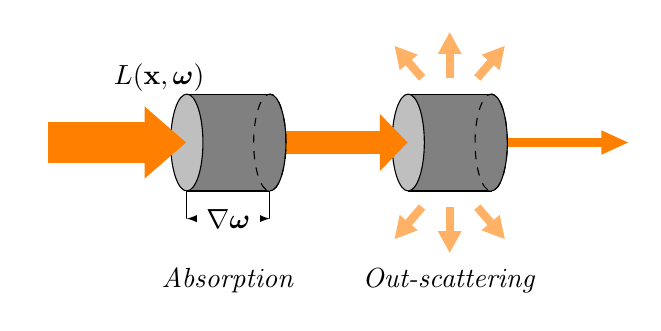
\begin{tikzpicture}
% 1 = 20p
    \def\XSTART{-40pt}
    \def\YSTART{60pt}
    \def\YDIAONE{35pt}
    \def\XONESTART{10pt}
    \def\XONEDELTA{30pt} %width of cylinders
    \def\DD{-10pt} %
    \def\GAP{50pt} %
    
    \def\LABELYSHIFT{-50pt}
    
    %FIRST cylinder
    \def\YEND{\YSTART+\YCURVE+\YDIATWO}
    \def\XONEEND{\XONESTART+\XONEDELTA}
    \def\YONEMIDDLE{\YSTART+\YDIAONE/2}
  
    %SECOND cylinder
    \def\XTWOSTART{\XONESTART+\XONEDELTA+\GAP}
    \def\XTWOEND{\XONEEND+\GAP+\XONEDELTA}
  
    %THIRD cylinder
    \def\XTHREESTART{\XONESTART+\XONEDELTA+\GAP+\XONEDELTA+\GAP}
    \def\XTHREEEND{\XONEEND+\GAP+\XONEDELTA+\GAP+\XONEDELTA}
    
    % FOURTH cylinder
    \def\XFOURSTART{\XONESTART+\XONEDELTA+\GAP+\XONEDELTA+\GAP+\XONEDELTA+\GAP}
    \def\XFOUREND{\XONEEND+\GAP+\XONEDELTA+\GAP+\XONEDELTA+\GAP+\XONEDELTA}

    \tikzset{
      partial ellipse/.style args={#1:#2:#3}{
          insert path={+ (#1:#3) arc (#1:#2:#3)}
      },
      dimen/.style={<->,>=latex,thin,
        every rectangle node/.style={fill=white,midway,font=\sffamily}},
    }

    % THIRD ARROW (OUT-SCATTERING)
    \draw[-{Triangle[width=8pt,length=10pt, color=orange]}, 
            line width=3pt, color=orange]
        (\XTWOEND+0.5,\YONEMIDDLE) -- ({\XTWOEND+\GAP-0.2},\YONEMIDDLE);
    
        % OUTSCATTERING ARROWS AROUND SECOND CYLINDER
    % above
    \draw[-{Triangle[width=8pt,length=8pt, color=orange!60]}, 
            line width=3pt, color=orange!60]
        ({\XTWOSTART+\XONEDELTA/2},{\YONEMIDDLE+\YDIAONE/1.5}) -- 
        ({\XTWOSTART+\XONEDELTA/2},{\YONEMIDDLE+40pt});
    \draw[-{Triangle[width=8pt,length=8pt, color=orange!60]}, 
            line width=3pt, color=orange!60]
        ({\XTWOSTART+\XONEDELTA/2-10pt},{\YONEMIDDLE+\YDIAONE/1.5}) -- 
        ({\XTWOSTART+\XONEDELTA/2-20pt},{\YONEMIDDLE+35pt});
    \draw[-{Triangle[width=8pt,length=8pt, color=orange!60]}, 
            line width=3pt, color=orange!60]
        ({\XTWOSTART+\XONEDELTA/2+10pt},{\YONEMIDDLE+\YDIAONE/1.5}) -- 
        ({\XTWOSTART+\XONEDELTA/2+20pt},{\YONEMIDDLE+35pt});
    % below
    \draw[-{Triangle[width=8pt,length=8pt, color=orange!60]}, 
            line width=3pt, color=orange!60]
        ({\XTWOSTART+\XONEDELTA/2},{\YONEMIDDLE-\YDIAONE/1.5}) -- 
        ({\XTWOSTART+\XONEDELTA/2},{\YONEMIDDLE-40pt});
    \draw[-{Triangle[width=8pt,length=8pt, color=orange!60]}, 
            line width=3pt, color=orange!60]
        ({\XTWOSTART+\XONEDELTA/2-10pt},{\YONEMIDDLE-\YDIAONE/1.5}) -- 
        ({\XTWOSTART+\XONEDELTA/2-20pt},{\YONEMIDDLE-35pt});
    \draw[-{Triangle[width=8pt,length=8pt, color=orange!60]}, 
            line width=3pt, color=orange!60]
        ({\XTWOSTART+\XONEDELTA/2+10pt},{\YONEMIDDLE-\YDIAONE/1.5}) -- 
        ({\XTWOSTART+\XONEDELTA/2+20pt},{\YONEMIDDLE-35pt});

    % SECOND CYLINDER
    \draw [fill=gray] (\XTWOSTART,\YSTART) coordinate (BA)
        rectangle (\XTWOEND,{\YSTART+\YDIAONE}) coordinate (BB);
    \draw [fill=lightgray](\XTWOSTART,\YONEMIDDLE)
        ellipse ({\YDIAONE/6} and {\YDIAONE/2});
    \draw [fill=gray,dashed](\XTWOEND,\YONEMIDDLE)
        ellipse ({\YDIAONE/6} and {\YDIAONE/2});
    \draw (\XTWOEND,\YONEMIDDLE)
        [partial ellipse=-90:90:{\YDIAONE/6} and {\YDIAONE/2}];

    \node[yshift=\LABELYSHIFT] at ($0.5*(BA)+0.5*(BB)$) {
        \textit{Out-scattering} 
    };

    
    % SECOND ARROW
    \draw[-{Triangle[width=20pt,length=10pt, color=orange]}, 
            line width=8pt, color=orange]
        ({\XONEEND+0.5},\YONEMIDDLE) -- ({\XONEEND+\GAP-0.2},\YONEMIDDLE);
    
    % FIRST CYLINDER
    \draw [fill=gray] (\XONESTART,\YSTART) coordinate (BA)
        rectangle (\XONEEND,{\YSTART+\YDIAONE}) coordinate (BB);
    \draw [fill=lightgray](\XONESTART,\YONEMIDDLE)
        ellipse ({\YDIAONE/6} and {\YDIAONE/2});
    \draw [fill=gray,dashed](\XONEEND,\YONEMIDDLE)
        ellipse ({\YDIAONE/6} and {\YDIAONE/2});
    \draw (\XONEEND,\YONEMIDDLE)
        [partial ellipse=-90:90:{\YDIAONE/6} and {\YDIAONE/2}];

    \node[yshift=\LABELYSHIFT] at ($0.5*(BA)+0.5*(BB)$) {
        \textit{Absorption} 
    };
    
    %nabla omega below
    \draw ($(BB)-(0,\YDIAONE)$) -- ++(0,\DD) coordinate (D1) -- +(0,5pt);
    \draw (BA) -- ++(0,\DD) coordinate (D2) -- +(0,5pt);
    \draw [dimen] (D1) -- (D2) node {$\nabla\boldsymbol\omega$};

    % INCOMING ARROW
    \draw[-{Triangle[width=25pt,length=15pt, color=orange]}, 
            line width=15pt, color=orange]
            node [above=85pt ] {$\textcolor{black}{L(\textbf{x},\boldsymbol\omega)}$}
        (\XSTART,\YONEMIDDLE) -- (\XONESTART-0.2,\YONEMIDDLE);


    %ground
    %\draw [fill=gray] (0,0) rectangle  (\XEND,\GROUND);

\end{tikzpicture}%

    \label{fig:interactions}
\end{figure}

\begin{columns}[t, onlytextwidth]
    \column{.49\textwidth}
    $\sigma_a$ : Absorption coefficient  \\
    $\sigma_s$ : Scattering coefficient \\
    $\sigma_a + \sigma_s = \sigma_t $ : Extinction coefficient
    \column{.49\textwidth}
    We lose 
    $\sigma_t(\bx)L(\bx, \bomega)$
    radiance \\ due to \textit{absorption} and \textit{out-scattering}.
    
\end{columns}
\vspace{3mm}


\end{frame}

\begin{frame}{In-scattered radiance}
\begin{figure}[ht]
    \centering
    \scalebox{.6}{
        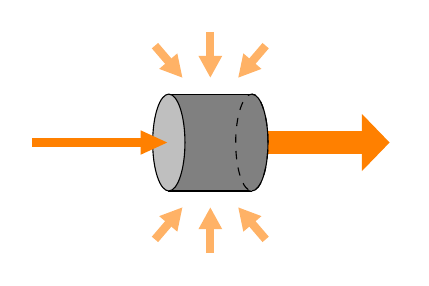
\begin{tikzpicture}
% 1 = 20p
    \def\XSTART{-40pt}
    \def\YSTART{60pt}
    \def\YDIAONE{35pt}
    \def\XONESTART{10pt}
    \def\XONEDELTA{30pt} %width of cylinders
    \def\DD{-10pt} %
    \def\GAP{50pt} %
    
    \def\LABELYSHIFT{-50pt}
    
    %FIRST cylinder
    \def\YEND{\YSTART+\YCURVE+\YDIATWO}
    \def\XONEEND{\XONESTART+\XONEDELTA}
    \def\YONEMIDDLE{\YSTART+\YDIAONE/2}
  
    %SECOND cylinder
    \def\XTWOSTART{\XONESTART+\XONEDELTA+\GAP}
    \def\XTWOEND{\XONEEND+\GAP+\XONEDELTA}
  
    %THIRD cylinder
    \def\XTHREESTART{\XONESTART+\XONEDELTA+\GAP+\XONEDELTA+\GAP}
    \def\XTHREEEND{\XONEEND+\GAP+\XONEDELTA+\GAP+\XONEDELTA}
    
    % FOURTH cylinder
    \def\XFOURSTART{\XONESTART+\XONEDELTA+\GAP+\XONEDELTA+\GAP+\XONEDELTA+\GAP}
    \def\XFOUREND{\XONEEND+\GAP+\XONEDELTA+\GAP+\XONEDELTA+\GAP+\XONEDELTA}

    \tikzset{
      partial ellipse/.style args={#1:#2:#3}{
          insert path={+ (#1:#3) arc (#1:#2:#3)}
      },
      dimen/.style={<->,>=latex,thin,
        every rectangle node/.style={fill=white,midway,font=\sffamily}},
    }
  
    % FIFTH ARROW (IN-SCATTERING)
    \draw[-{Triangle[width=20pt,length=10pt, color=orange]}, 
            line width=8pt, color=orange]
        (\XTHREEEND+0.5,\YONEMIDDLE) -- (\XTHREEEND+\GAP-0.2,\YONEMIDDLE);
    

    % INSCATTERING ARROWS AROUND THIRD CYLINDER
    % above
    \draw[-{Triangle[width=8pt,length=8pt, color=orange!60]}, 
            line width=3pt, color=orange!60]
        ({\XTHREESTART+\XONEDELTA/2},{\YONEMIDDLE+40pt}) --
        ({\XTHREESTART+\XONEDELTA/2},{\YONEMIDDLE+\YDIAONE/1.5});
    \draw[-{Triangle[width=8pt,length=8pt, color=orange!60]}, 
            line width=3pt, color=orange!60]
        ({\XTHREESTART+\XONEDELTA/2-20pt},{\YONEMIDDLE+35pt}) --
        ({\XTHREESTART+\XONEDELTA/2-10pt},{\YONEMIDDLE+\YDIAONE/1.5});
    \draw[-{Triangle[width=8pt,length=8pt, color=orange!60]}, 
            line width=3pt, color=orange!60]
        ({\XTHREESTART+\XONEDELTA/2+20pt},{\YONEMIDDLE+35pt}) --
        ({\XTHREESTART+\XONEDELTA/2+10pt},{\YONEMIDDLE+\YDIAONE/1.5});
    % below
    \draw[-{Triangle[width=8pt,length=8pt, color=orange!60]}, 
            line width=3pt, color=orange!60]
        ({\XTHREESTART+\XONEDELTA/2},{\YONEMIDDLE-40pt}) --
        ({\XTHREESTART+\XONEDELTA/2},{\YONEMIDDLE-\YDIAONE/1.5});
    \draw[-{Triangle[width=8pt,length=8pt, color=orange!60]}, 
            line width=3pt, color=orange!60]
        ({\XTHREESTART+\XONEDELTA/2-20pt},{\YONEMIDDLE-35pt}) -- 
        ({\XTHREESTART+\XONEDELTA/2-10pt},{\YONEMIDDLE-\YDIAONE/1.5});
    \draw[-{Triangle[width=8pt,length=8pt, color=orange!60]}, 
            line width=3pt, color=orange!60]
        ({\XTHREESTART+\XONEDELTA/2+20pt},{\YONEMIDDLE-35pt}) --
        ({\XTHREESTART+\XONEDELTA/2+10pt},{\YONEMIDDLE-\YDIAONE/1.5});

    \draw [fill=gray] (\XTHREESTART,\YSTART) coordinate (BA)
        rectangle (\XTHREEEND,{\YSTART+\YDIAONE}) coordinate (BB);
    \draw [fill=lightgray](\XTHREESTART,\YONEMIDDLE)
        ellipse ({\YDIAONE/6} and {\YDIAONE/2});
    \draw [fill=gray,dashed](\XTHREEEND,\YONEMIDDLE)
        ellipse ({\YDIAONE/6} and {\YDIAONE/2});
    \draw (\XTHREEEND,\YONEMIDDLE)
        [partial ellipse=-90:90:{\YDIAONE/6} and {\YDIAONE/2}];

    % \node[yshift=\LABELYSHIFT] at ($0.5*(BA)+0.5*(BB)$) {\textit{In-scattering}};

    % THIRD ARROW (OUT-SCATTERING)
    \draw[-{Triangle[width=8pt,length=10pt, color=orange]}, 
            line width=3pt, color=orange]
        (\XTWOEND+0.5,\YONEMIDDLE) -- ({\XTWOEND+\GAP-0.2},\YONEMIDDLE);
    

\end{tikzpicture}%

    }
\end{figure}
$$ L_s(\bx, \bomega) = \int_{S^2} f_p(\bx, \bomega, \bomega') L_i(\bx, \bomega')
    d\bomega' $$

\begin{columns}[t, onlytextwidth]
    \column{.20\textwidth}
    Phase function $f_p(\bx, \bomega, \bomega')$ \\
    \vspace{.3em}
    \scriptsize{$\approx BSDF$ \\(in surface rendering)}
    \column{.79\textwidth}
    \begin{itemize}
        \item scattering at point $\bx$, given incident ($\bomega$) and outgoing
            ($\bomega'$) directions
        \item $\int_{S^2} f_p = 1$
        \item $f_p(\theta)\big|_{\theta = \measuredangle(\bomega, \bomega')}$
        \item $f_p(\bx, \bomega, \bomega') = 1/(4\pi)$, if the medium is
            \textit{isotropic}\\\hfill(otherwise, \textit{anisotropic})
    \end{itemize}
\end{columns}

\end{frame}


\begin{frame}{Emission}
\begin{figure}[ht]
    \centering
    % \scalebox{.7}{
        
\begin{tikzpicture}
% 1 = 20p
    \def\XSTART{-40pt}
    \def\YSTART{60pt}
    \def\YDIAONE{35pt}
    \def\XONESTART{10pt}
    \def\XONEDELTA{30pt} %width of cylinders
    \def\DD{-10pt} %
    \def\GAP{50pt} %
    
    \def\LABELYSHIFT{-50pt}
    
    %FIRST cylinder
    \def\YEND{\YSTART+\YCURVE+\YDIATWO}
    \def\XONEEND{\XONESTART+\XONEDELTA}
    \def\YONEMIDDLE{\YSTART+\YDIAONE/2}
  
    %SECOND cylinder
    \def\XTWOSTART{\XONESTART+\XONEDELTA+\GAP}
    \def\XTWOEND{\XONEEND+\GAP+\XONEDELTA}
  
    %THIRD cylinder
    \def\XTHREESTART{\XONESTART+\XONEDELTA+\GAP+\XONEDELTA+\GAP}
    \def\XTHREEEND{\XONEEND+\GAP+\XONEDELTA+\GAP+\XONEDELTA}
    
    % FOURTH cylinder
    \def\XFOURSTART{\XONESTART+\XONEDELTA+\GAP+\XONEDELTA+\GAP+\XONEDELTA+\GAP}
    \def\XFOUREND{\XONEEND+\GAP+\XONEDELTA+\GAP+\XONEDELTA+\GAP+\XONEDELTA}

    \tikzset{
      partial ellipse/.style args={#1:#2:#3}{
          insert path={+ (#1:#3) arc (#1:#2:#3)}
      },
      dimen/.style={<->,>=latex,thin,
        every rectangle node/.style={fill=white,midway,font=\sffamily}},
    }
  
    % OUTGOING ARROW (EMISSION)
    \draw[-{Triangle[width=25pt,length=15pt, color=orange]}, 
            line width=15pt, color=orange]
        (\XFOUREND+0.5,\YONEMIDDLE) -- (\XFOUREND+\GAP,\YONEMIDDLE);

    %FOURTH CYLINDER
    \draw [fill=gray] (\XFOURSTART,\YSTART) coordinate (BA)
        rectangle (\XFOUREND,{\YSTART+\YDIAONE}) coordinate (BB);
    \draw [fill=lightgray](\XFOURSTART,\YONEMIDDLE)
        ellipse ({\YDIAONE/6} and {\YDIAONE/2});
    \draw [fill=gray,dashed](\XFOUREND,\YONEMIDDLE)
        ellipse ({\YDIAONE/6} and {\YDIAONE/2});
    \draw (\XFOUREND,\YONEMIDDLE)
        [partial ellipse=-90:90:{\YDIAONE/6} and {\YDIAONE/2}];

    % \node[yshift=\LABELYSHIFT] at ($0.5*(BA)+0.5*(BB)$) {\textit{Emission}};

    % FIFTH ARROW (IN-SCATTERING)
    \draw[-{Triangle[width=20pt,length=10pt, color=orange]}, 
            line width=8pt, color=orange]
        (\XTHREEEND+0.5,\YONEMIDDLE) -- (\XTHREEEND+\GAP-0.2,\YONEMIDDLE);
    


\end{tikzpicture}%

    % }
\end{figure}
$$L_e(\bx, \bomega)$$

$$\sigma_a(\boldsymbol{x})L_e(\bx, \bomega)$$
\end{frame}

%\section{Second Section}
\begin{frame}{Assembling all the parts}
    \begin{figure}[ht]
        \centering
        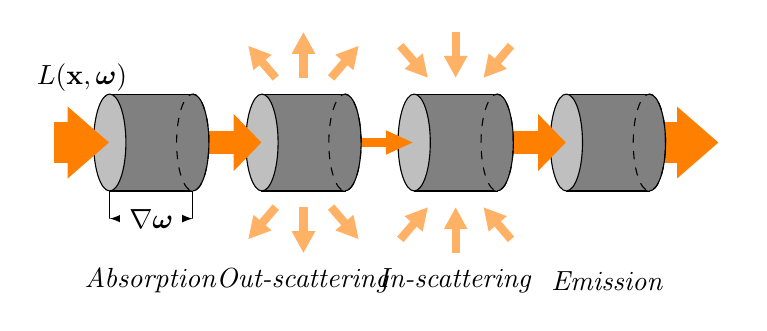
\begin{tikzpicture}
% 1 = 20p
    \def\XSTART{-10pt}
    \def\YSTART{60pt}
    \def\YDIAONE{35pt}
    \def\XONESTART{10pt}
    \def\XONEDELTA{30pt} %width of cylinders
    \def\DD{-10pt} %
    \def\GAP{25pt} %
    
    \def\LABELYSHIFT{-50pt}
    
    %FIRST cylinder
    \def\YEND{\YSTART+\YCURVE+\YDIATWO}
    \def\XONEEND{\XONESTART+\XONEDELTA}
    \def\YONEMIDDLE{\YSTART+\YDIAONE/2}
  
    %SECOND cylinder
    \def\XTWOSTART{\XONESTART+\XONEDELTA+\GAP}
    \def\XTWOEND{\XONEEND+\GAP+\XONEDELTA}
  
    %THIRD cylinder
    \def\XTHREESTART{\XONESTART+\XONEDELTA+\GAP+\XONEDELTA+\GAP}
    \def\XTHREEEND{\XONEEND+\GAP+\XONEDELTA+\GAP+\XONEDELTA}
    
    % FOURTH cylinder
    \def\XFOURSTART{\XONESTART+\XONEDELTA+\GAP+\XONEDELTA+\GAP+\XONEDELTA+\GAP}
    \def\XFOUREND{\XONEEND+\GAP+\XONEDELTA+\GAP+\XONEDELTA+\GAP+\XONEDELTA}

    \tikzset{
      partial ellipse/.style args={#1:#2:#3}{
          insert path={+ (#1:#3) arc (#1:#2:#3)}
      },
      dimen/.style={<->,>=latex,thin,
        every rectangle node/.style={fill=white,midway,font=\sffamily}},
    }
  
    % OUTGOING ARROW (EMISSION)
    \draw[-{Triangle[width=25pt,length=15pt, color=orange]}, 
            line width=15pt, color=orange]
        (\XFOUREND+0.5,\YONEMIDDLE) -- (\XFOUREND+\GAP,\YONEMIDDLE);

    %FOURTH CYLINDER
    \draw [fill=gray] (\XFOURSTART,\YSTART) coordinate (BA)
        rectangle (\XFOUREND,{\YSTART+\YDIAONE}) coordinate (BB);
    \draw [fill=lightgray](\XFOURSTART,\YONEMIDDLE)
        ellipse ({\YDIAONE/6} and {\YDIAONE/2});
    \draw [fill=gray,dashed](\XFOUREND,\YONEMIDDLE)
        ellipse ({\YDIAONE/6} and {\YDIAONE/2});
    \draw (\XFOUREND,\YONEMIDDLE)
        [partial ellipse=-90:90:{\YDIAONE/6} and {\YDIAONE/2}];

    \node[yshift=\LABELYSHIFT] at ($0.5*(BA)+0.5*(BB)$) {\textit{Emission}};

    % FIFTH ARROW (IN-SCATTERING)
    \draw[-{Triangle[width=20pt,length=10pt, color=orange]}, 
            line width=8pt, color=orange]
        (\XTHREEEND+0.5,\YONEMIDDLE) -- (\XTHREEEND+\GAP-0.2,\YONEMIDDLE);
    

    % INSCATTERING ARROWS AROUND THIRD CYLINDER
    % above
    \draw[-{Triangle[width=8pt,length=8pt, color=orange!60]}, 
            line width=3pt, color=orange!60]
        ({\XTHREESTART+\XONEDELTA/2},{\YONEMIDDLE+40pt}) --
        ({\XTHREESTART+\XONEDELTA/2},{\YONEMIDDLE+\YDIAONE/1.5});
    \draw[-{Triangle[width=8pt,length=8pt, color=orange!60]}, 
            line width=3pt, color=orange!60]
        ({\XTHREESTART+\XONEDELTA/2-20pt},{\YONEMIDDLE+35pt}) --
        ({\XTHREESTART+\XONEDELTA/2-10pt},{\YONEMIDDLE+\YDIAONE/1.5});
    \draw[-{Triangle[width=8pt,length=8pt, color=orange!60]}, 
            line width=3pt, color=orange!60]
        ({\XTHREESTART+\XONEDELTA/2+20pt},{\YONEMIDDLE+35pt}) --
        ({\XTHREESTART+\XONEDELTA/2+10pt},{\YONEMIDDLE+\YDIAONE/1.5});
    % below
    \draw[-{Triangle[width=8pt,length=8pt, color=orange!60]}, 
            line width=3pt, color=orange!60]
        ({\XTHREESTART+\XONEDELTA/2},{\YONEMIDDLE-40pt}) --
        ({\XTHREESTART+\XONEDELTA/2},{\YONEMIDDLE-\YDIAONE/1.5});
    \draw[-{Triangle[width=8pt,length=8pt, color=orange!60]}, 
            line width=3pt, color=orange!60]
        ({\XTHREESTART+\XONEDELTA/2-20pt},{\YONEMIDDLE-35pt}) -- 
        ({\XTHREESTART+\XONEDELTA/2-10pt},{\YONEMIDDLE-\YDIAONE/1.5});
    \draw[-{Triangle[width=8pt,length=8pt, color=orange!60]}, 
            line width=3pt, color=orange!60]
        ({\XTHREESTART+\XONEDELTA/2+20pt},{\YONEMIDDLE-35pt}) --
        ({\XTHREESTART+\XONEDELTA/2+10pt},{\YONEMIDDLE-\YDIAONE/1.5});

    \draw [fill=gray] (\XTHREESTART,\YSTART) coordinate (BA)
        rectangle (\XTHREEEND,{\YSTART+\YDIAONE}) coordinate (BB);
    \draw [fill=lightgray](\XTHREESTART,\YONEMIDDLE)
        ellipse ({\YDIAONE/6} and {\YDIAONE/2});
    \draw [fill=gray,dashed](\XTHREEEND,\YONEMIDDLE)
        ellipse ({\YDIAONE/6} and {\YDIAONE/2});
    \draw (\XTHREEEND,\YONEMIDDLE)
        [partial ellipse=-90:90:{\YDIAONE/6} and {\YDIAONE/2}];

    \node[yshift=\LABELYSHIFT] at ($0.5*(BA)+0.5*(BB)$) {\textit{In-scattering}};

    % THIRD ARROW (OUT-SCATTERING)
    \draw[-{Triangle[width=8pt,length=10pt, color=orange]}, 
            line width=3pt, color=orange]
        (\XTWOEND+0.5,\YONEMIDDLE) -- ({\XTWOEND+\GAP-0.2},\YONEMIDDLE);
    
        % OUTSCATTERING ARROWS AROUND SECOND CYLINDER
    % above
    \draw[-{Triangle[width=8pt,length=8pt, color=orange!60]}, 
            line width=3pt, color=orange!60]
        ({\XTWOSTART+\XONEDELTA/2},{\YONEMIDDLE+\YDIAONE/1.5}) -- 
        ({\XTWOSTART+\XONEDELTA/2},{\YONEMIDDLE+40pt});
    \draw[-{Triangle[width=8pt,length=8pt, color=orange!60]}, 
            line width=3pt, color=orange!60]
        ({\XTWOSTART+\XONEDELTA/2-10pt},{\YONEMIDDLE+\YDIAONE/1.5}) -- 
        ({\XTWOSTART+\XONEDELTA/2-20pt},{\YONEMIDDLE+35pt});
    \draw[-{Triangle[width=8pt,length=8pt, color=orange!60]}, 
            line width=3pt, color=orange!60]
        ({\XTWOSTART+\XONEDELTA/2+10pt},{\YONEMIDDLE+\YDIAONE/1.5}) -- 
        ({\XTWOSTART+\XONEDELTA/2+20pt},{\YONEMIDDLE+35pt});
    % below
    \draw[-{Triangle[width=8pt,length=8pt, color=orange!60]}, 
            line width=3pt, color=orange!60]
        ({\XTWOSTART+\XONEDELTA/2},{\YONEMIDDLE-\YDIAONE/1.5}) -- 
        ({\XTWOSTART+\XONEDELTA/2},{\YONEMIDDLE-40pt});
    \draw[-{Triangle[width=8pt,length=8pt, color=orange!60]}, 
            line width=3pt, color=orange!60]
        ({\XTWOSTART+\XONEDELTA/2-10pt},{\YONEMIDDLE-\YDIAONE/1.5}) -- 
        ({\XTWOSTART+\XONEDELTA/2-20pt},{\YONEMIDDLE-35pt});
    \draw[-{Triangle[width=8pt,length=8pt, color=orange!60]}, 
            line width=3pt, color=orange!60]
        ({\XTWOSTART+\XONEDELTA/2+10pt},{\YONEMIDDLE-\YDIAONE/1.5}) -- 
        ({\XTWOSTART+\XONEDELTA/2+20pt},{\YONEMIDDLE-35pt});

    % SECOND CYLINDER
    \draw [fill=gray] (\XTWOSTART,\YSTART) coordinate (BA)
        rectangle (\XTWOEND,{\YSTART+\YDIAONE}) coordinate (BB);
    \draw [fill=lightgray](\XTWOSTART,\YONEMIDDLE)
        ellipse ({\YDIAONE/6} and {\YDIAONE/2});
    \draw [fill=gray,dashed](\XTWOEND,\YONEMIDDLE)
        ellipse ({\YDIAONE/6} and {\YDIAONE/2});
    \draw (\XTWOEND,\YONEMIDDLE)
        [partial ellipse=-90:90:{\YDIAONE/6} and {\YDIAONE/2}];

    \node[yshift=\LABELYSHIFT] at ($0.5*(BA)+0.5*(BB)$) {\textit{Out-scattering}};
    
    % SECOND ARROW
    \draw[-{Triangle[width=20pt,length=10pt, color=orange]}, 
            line width=8pt, color=orange]
        ({\XONEEND+0.5},\YONEMIDDLE) -- ({\XONEEND+\GAP-0.2},\YONEMIDDLE);
    
    % FIRST CYLINDER
    \draw [fill=gray] (\XONESTART,\YSTART) coordinate (BA)
        rectangle (\XONEEND,{\YSTART+\YDIAONE}) coordinate (BB);
    \draw [fill=lightgray](\XONESTART,\YONEMIDDLE)
        ellipse ({\YDIAONE/6} and {\YDIAONE/2});
    \draw [fill=gray,dashed](\XONEEND,\YONEMIDDLE)
        ellipse ({\YDIAONE/6} and {\YDIAONE/2});
    \draw (\XONEEND,\YONEMIDDLE)
        [partial ellipse=-90:90:{\YDIAONE/6} and {\YDIAONE/2}];

    \node[yshift=\LABELYSHIFT] at ($0.5*(BA)+0.5*(BB)$) {\textit{Absorption}};
    
    %nabla omega below
    \draw ($(BB)-(0,\YDIAONE)$) -- ++(0,\DD) coordinate (D1) -- +(0,5pt);
    \draw (BA) -- ++(0,\DD) coordinate (D2) -- +(0,5pt);
    \draw [dimen] (D1) -- (D2) node {$\nabla\boldsymbol\omega$};

    % INCOMING ARROW
    \draw[-{Triangle[width=25pt,length=15pt, color=orange]}, 
            line width=15pt, color=orange]
            node [above=85pt ] {$\textcolor{black}{L(\textbf{x},\boldsymbol\omega)}$}
        (\XSTART,\YONEMIDDLE) -- (\XONESTART-0.2,\YONEMIDDLE);


    %ground
    %\draw [fill=gray] (0,0) rectangle  (\XEND,\GROUND);

\end{tikzpicture}%

        \label{fig:interactions}
    \end{figure}
    \begin{itemize}
        \item Loses $\sigma_a L(x, \omega)$ due to absorption
        \item Loses $\sigma_s L(x, \omega)$ due to out-scattering
        \item Gains $\sigma_s L_i(x, \omega)$ due to in-scattering
        \item Gains $\sigma_a L_e(x, \omega)$ due to emission
    \end{itemize}
\end{frame}


\begin{frame}{RTE -- Radiative Transfer Equation}
    The change in radiance $L$ traveling along direction $\boldsymbol{\omega}$
    through a differential volume element at point $\boldsymbol{x}$.
    \begin{figure}[ht]
        \centering
        \scalebox{.7}{
            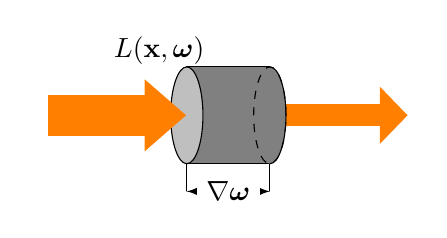
\begin{tikzpicture}
% 1 = 20p
    \def\XSTART{-40pt}
    \def\YSTART{60pt}
    \def\YDIAONE{35pt}
    \def\XONESTART{10pt}
    \def\XONEDELTA{30pt} %width of cylinders
    \def\DD{-10pt} %
    \def\GAP{50pt} %
    
    \def\LABELYSHIFT{-50pt}
    
    %FIRST cylinder
    \def\YEND{\YSTART+\YCURVE+\YDIATWO}
    \def\XONEEND{\XONESTART+\XONEDELTA}
    \def\YONEMIDDLE{\YSTART+\YDIAONE/2}
  
    %SECOND cylinder
    \def\XTWOSTART{\XONESTART+\XONEDELTA+\GAP}
    \def\XTWOEND{\XONEEND+\GAP+\XONEDELTA}
  
    %THIRD cylinder
    \def\XTHREESTART{\XONESTART+\XONEDELTA+\GAP+\XONEDELTA+\GAP}
    \def\XTHREEEND{\XONEEND+\GAP+\XONEDELTA+\GAP+\XONEDELTA}
    
    % FOURTH cylinder
    \def\XFOURSTART{\XONESTART+\XONEDELTA+\GAP+\XONEDELTA+\GAP+\XONEDELTA+\GAP}
    \def\XFOUREND{\XONEEND+\GAP+\XONEDELTA+\GAP+\XONEDELTA+\GAP+\XONEDELTA}

    \tikzset{
      partial ellipse/.style args={#1:#2:#3}{
          insert path={+ (#1:#3) arc (#1:#2:#3)}
      },
      dimen/.style={<->,>=latex,thin,
        every rectangle node/.style={fill=white,midway,font=\sffamily}},
    }
  
    
    % SECOND ARROW
    \draw[-{Triangle[width=20pt,length=10pt, color=orange]}, 
            line width=8pt, color=orange]
        ({\XONEEND+0.5},\YONEMIDDLE) -- ({\XONEEND+\GAP-0.2},\YONEMIDDLE);
    
    % FIRST CYLINDER
    \draw [fill=gray] (\XONESTART,\YSTART) coordinate (BA)
        rectangle (\XONEEND,{\YSTART+\YDIAONE}) coordinate (BB);
    \draw [fill=lightgray](\XONESTART,\YONEMIDDLE)
        ellipse ({\YDIAONE/6} and {\YDIAONE/2});
    \draw [fill=gray,dashed](\XONEEND,\YONEMIDDLE)
        ellipse ({\YDIAONE/6} and {\YDIAONE/2});
    \draw (\XONEEND,\YONEMIDDLE)
        [partial ellipse=-90:90:{\YDIAONE/6} and {\YDIAONE/2}];

    % \node[yshift=\LABELYSHIFT] at ($0.5*(BA)+0.5*(BB)$) {\textit{Absorption}};
    
    %nabla omega below
    \draw ($(BB)-(0,\YDIAONE)$) -- ++(0,\DD) coordinate (D1) -- +(0,5pt);
    \draw (BA) -- ++(0,\DD) coordinate (D2) -- +(0,5pt);
    \draw [dimen] (D1) -- (D2) node {$\nabla\boldsymbol\omega$};

    % INCOMING ARROW
    \draw[-{Triangle[width=25pt,length=15pt, color=orange]}, 
            line width=15pt, color=orange]
            node [above=85pt ] {$\textcolor{black}{L(\textbf{x},\boldsymbol\omega)}$}
        (\XSTART,\YONEMIDDLE) -- (\XONESTART-0.2,\YONEMIDDLE);


    %ground
    %\draw [fill=gray] (0,0) rectangle  (\XEND,\GROUND);

\end{tikzpicture}%

        }
    \end{figure}
    \begin{equation} 
        \label{eq:RTE}
        (\bomega \nabla)L(\bx,\bomega) =
        - \sigma_t(\bx)L(\bx,\bomega)
        + \sigma_s(\bx)L_s(\bx,\bomega) + \sigma_a(\bx)L_e(\bx,\bomega)
    \end{equation}
\end{frame}

\begin{frame}{RTE -- Radiative Transfer Equation}
    The change in radiance $L$ traveling along direction $\boldsymbol{\omega}$
    through a differential volume element at point $\boldsymbol{x}$.
    \begin{figure}[ht]
        \centering
        \scalebox{.7}{
            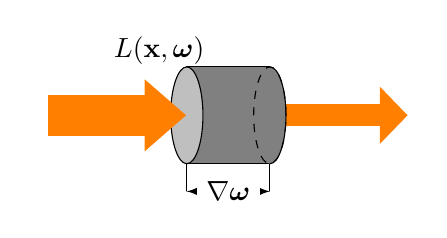
\begin{tikzpicture}
% 1 = 20p
    \def\XSTART{-40pt}
    \def\YSTART{60pt}
    \def\YDIAONE{35pt}
    \def\XONESTART{10pt}
    \def\XONEDELTA{30pt} %width of cylinders
    \def\DD{-10pt} %
    \def\GAP{50pt} %
    
    \def\LABELYSHIFT{-50pt}
    
    %FIRST cylinder
    \def\YEND{\YSTART+\YCURVE+\YDIATWO}
    \def\XONEEND{\XONESTART+\XONEDELTA}
    \def\YONEMIDDLE{\YSTART+\YDIAONE/2}
  
    %SECOND cylinder
    \def\XTWOSTART{\XONESTART+\XONEDELTA+\GAP}
    \def\XTWOEND{\XONEEND+\GAP+\XONEDELTA}
  
    %THIRD cylinder
    \def\XTHREESTART{\XONESTART+\XONEDELTA+\GAP+\XONEDELTA+\GAP}
    \def\XTHREEEND{\XONEEND+\GAP+\XONEDELTA+\GAP+\XONEDELTA}
    
    % FOURTH cylinder
    \def\XFOURSTART{\XONESTART+\XONEDELTA+\GAP+\XONEDELTA+\GAP+\XONEDELTA+\GAP}
    \def\XFOUREND{\XONEEND+\GAP+\XONEDELTA+\GAP+\XONEDELTA+\GAP+\XONEDELTA}

    \tikzset{
      partial ellipse/.style args={#1:#2:#3}{
          insert path={+ (#1:#3) arc (#1:#2:#3)}
      },
      dimen/.style={<->,>=latex,thin,
        every rectangle node/.style={fill=white,midway,font=\sffamily}},
    }
  
    
    % SECOND ARROW
    \draw[-{Triangle[width=20pt,length=10pt, color=orange]}, 
            line width=8pt, color=orange]
        ({\XONEEND+0.5},\YONEMIDDLE) -- ({\XONEEND+\GAP-0.2},\YONEMIDDLE);
    
    % FIRST CYLINDER
    \draw [fill=gray] (\XONESTART,\YSTART) coordinate (BA)
        rectangle (\XONEEND,{\YSTART+\YDIAONE}) coordinate (BB);
    \draw [fill=lightgray](\XONESTART,\YONEMIDDLE)
        ellipse ({\YDIAONE/6} and {\YDIAONE/2});
    \draw [fill=gray,dashed](\XONEEND,\YONEMIDDLE)
        ellipse ({\YDIAONE/6} and {\YDIAONE/2});
    \draw (\XONEEND,\YONEMIDDLE)
        [partial ellipse=-90:90:{\YDIAONE/6} and {\YDIAONE/2}];

    % \node[yshift=\LABELYSHIFT] at ($0.5*(BA)+0.5*(BB)$) {\textit{Absorption}};
    
    %nabla omega below
    \draw ($(BB)-(0,\YDIAONE)$) -- ++(0,\DD) coordinate (D1) -- +(0,5pt);
    \draw (BA) -- ++(0,\DD) coordinate (D2) -- +(0,5pt);
    \draw [dimen] (D1) -- (D2) node {$\nabla\boldsymbol\omega$};

    % INCOMING ARROW
    \draw[-{Triangle[width=25pt,length=15pt, color=orange]}, 
            line width=15pt, color=orange]
            node [above=85pt ] {$\textcolor{black}{L(\textbf{x},\boldsymbol\omega)}$}
        (\XSTART,\YONEMIDDLE) -- (\XONESTART-0.2,\YONEMIDDLE);


    %ground
    %\draw [fill=gray] (0,0) rectangle  (\XEND,\GROUND);

\end{tikzpicture}%

        }
    \end{figure}
    \begin{equation} 
        \label{eq:RTE}
        (\bomega \nabla)L(\bx,\bomega) =
        - \sigma_t(\bx)L(\bx,\bomega)
        + \sigma_s(\bx)L_s(\bx,\bomega) + \sigma_a(\bx)L_e(\bx,\bomega)
    \end{equation}
    \centering
    \vfill
    \textbf{Let's integrate it!}
\end{frame}

\begin{frame}{Integrating the loss of radiance}
\begin{figure}[ht]
    \centering
    \scalebox{.6}{
        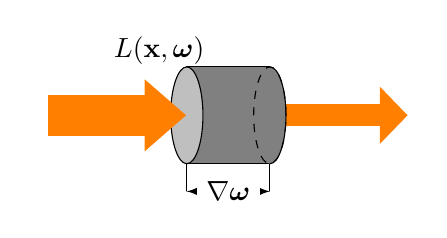
\begin{tikzpicture}
% 1 = 20p
    \def\XSTART{-40pt}
    \def\YSTART{60pt}
    \def\YDIAONE{35pt}
    \def\XONESTART{10pt}
    \def\XONEDELTA{30pt} %width of cylinders
    \def\DD{-10pt} %
    \def\GAP{50pt} %
    
    \def\LABELYSHIFT{-50pt}
    
    %FIRST cylinder
    \def\YEND{\YSTART+\YCURVE+\YDIATWO}
    \def\XONEEND{\XONESTART+\XONEDELTA}
    \def\YONEMIDDLE{\YSTART+\YDIAONE/2}
  
    %SECOND cylinder
    \def\XTWOSTART{\XONESTART+\XONEDELTA+\GAP}
    \def\XTWOEND{\XONEEND+\GAP+\XONEDELTA}
  
    %THIRD cylinder
    \def\XTHREESTART{\XONESTART+\XONEDELTA+\GAP+\XONEDELTA+\GAP}
    \def\XTHREEEND{\XONEEND+\GAP+\XONEDELTA+\GAP+\XONEDELTA}
    
    % FOURTH cylinder
    \def\XFOURSTART{\XONESTART+\XONEDELTA+\GAP+\XONEDELTA+\GAP+\XONEDELTA+\GAP}
    \def\XFOUREND{\XONEEND+\GAP+\XONEDELTA+\GAP+\XONEDELTA+\GAP+\XONEDELTA}

    \tikzset{
      partial ellipse/.style args={#1:#2:#3}{
          insert path={+ (#1:#3) arc (#1:#2:#3)}
      },
      dimen/.style={<->,>=latex,thin,
        every rectangle node/.style={fill=white,midway,font=\sffamily}},
    }
  
    
    % SECOND ARROW
    \draw[-{Triangle[width=20pt,length=10pt, color=orange]}, 
            line width=8pt, color=orange]
        ({\XONEEND+0.5},\YONEMIDDLE) -- ({\XONEEND+\GAP-0.2},\YONEMIDDLE);
    
    % FIRST CYLINDER
    \draw [fill=gray] (\XONESTART,\YSTART) coordinate (BA)
        rectangle (\XONEEND,{\YSTART+\YDIAONE}) coordinate (BB);
    \draw [fill=lightgray](\XONESTART,\YONEMIDDLE)
        ellipse ({\YDIAONE/6} and {\YDIAONE/2});
    \draw [fill=gray,dashed](\XONEEND,\YONEMIDDLE)
        ellipse ({\YDIAONE/6} and {\YDIAONE/2});
    \draw (\XONEEND,\YONEMIDDLE)
        [partial ellipse=-90:90:{\YDIAONE/6} and {\YDIAONE/2}];

    % \node[yshift=\LABELYSHIFT] at ($0.5*(BA)+0.5*(BB)$) {\textit{Absorption}};
    
    %nabla omega below
    \draw ($(BB)-(0,\YDIAONE)$) -- ++(0,\DD) coordinate (D1) -- +(0,5pt);
    \draw (BA) -- ++(0,\DD) coordinate (D2) -- +(0,5pt);
    \draw [dimen] (D1) -- (D2) node {$\nabla\boldsymbol\omega$};

    % INCOMING ARROW
    \draw[-{Triangle[width=25pt,length=15pt, color=orange]}, 
            line width=15pt, color=orange]
            node [above=85pt ] {$\textcolor{black}{L(\textbf{x},\boldsymbol\omega)}$}
        (\XSTART,\YONEMIDDLE) -- (\XONESTART-0.2,\YONEMIDDLE);


    %ground
    %\draw [fill=gray] (0,0) rectangle  (\XEND,\GROUND);

\end{tikzpicture}%

    }
    \begin{align}
    \begin{aligned}
        % \vert\nabla\bomega\vert &=  \\
        L(\bx + \nabla\bomega,\bomega) &= 
            L(\bx,\bomega) - \sigma_t(\bx)L(\bx,\bomega)\nabla\bomega \\ 
        L(\bx + dx) &= 
            L(\bx) - L(\bx)\sigma_t(\bx)dx\bigg|_{dx=\nabla\bomega,
            L(\bx)=L(\bx, \bomega)} \\
        \frac{L(\bx + dx) - L(\bx)}{dx} = \Aboxed{\frac{dL(\bx)}{dx} &=
        -L(\bx)\sigma_t(\bx)} \text{ ("exponential extinction")}\\
        \int_{L(x)}^{L(x+S)} \frac{1}{L} dL &= -\int_0^S \sigma_t(\bx)dx\\
        ln(L(\bx+S)) - ln(L(\bx)) &= - \int_0^S \sigma_t(\bx) dx
    \end{aligned}
    \end{align}
\end{figure}
\end{frame}


\begin{frame}{Transmittance}{The Beer-Lambert Law}
\begin{figure}[ht]
$$ \implies L(\bx + S) = L(\bx)e^{-\int_0^S \sigma_t(\bx+s)ds} $$
\end{figure}

Usually written as:\\
\begin{columns}[t, onlytextwidth]
\column{.49\textwidth}
    $e^{-\int_0^y \sigma_t(\bx-s\bomega)ds} = T(\bx, \by)$
    \\
    \textit{"transmittance coefficient"} $T(\bx, \by)$\\
    net reduction factor between $\bx$ and $\by$ \\due to absorption and
    out-scattering
\column{.49\textwidth}
    $\int_0^y \sigma_t(\bx-s\bomega)ds = \tau(\bx,\by)$\\
    \textit{"optical thickness" $\tau$}
\end{columns}

\vfill
$$ T(t) = e^{-\tau(t)} = e^{-\int_0^t \sigma_t(\bx-s\bomega)ds} $$
    \centering over distance $t$

\end{frame}

\begin{frame}{RTE -- Radiative Transfer Equation}
    {The integral version}
    \vfill
    % \begin{figure}[ht]
    %     \centering
    %     \scalebox{.7}{
    %         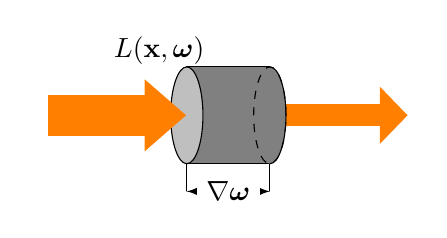
\begin{tikzpicture}
% 1 = 20p
    \def\XSTART{-40pt}
    \def\YSTART{60pt}
    \def\YDIAONE{35pt}
    \def\XONESTART{10pt}
    \def\XONEDELTA{30pt} %width of cylinders
    \def\DD{-10pt} %
    \def\GAP{50pt} %
    
    \def\LABELYSHIFT{-50pt}
    
    %FIRST cylinder
    \def\YEND{\YSTART+\YCURVE+\YDIATWO}
    \def\XONEEND{\XONESTART+\XONEDELTA}
    \def\YONEMIDDLE{\YSTART+\YDIAONE/2}
  
    %SECOND cylinder
    \def\XTWOSTART{\XONESTART+\XONEDELTA+\GAP}
    \def\XTWOEND{\XONEEND+\GAP+\XONEDELTA}
  
    %THIRD cylinder
    \def\XTHREESTART{\XONESTART+\XONEDELTA+\GAP+\XONEDELTA+\GAP}
    \def\XTHREEEND{\XONEEND+\GAP+\XONEDELTA+\GAP+\XONEDELTA}
    
    % FOURTH cylinder
    \def\XFOURSTART{\XONESTART+\XONEDELTA+\GAP+\XONEDELTA+\GAP+\XONEDELTA+\GAP}
    \def\XFOUREND{\XONEEND+\GAP+\XONEDELTA+\GAP+\XONEDELTA+\GAP+\XONEDELTA}

    \tikzset{
      partial ellipse/.style args={#1:#2:#3}{
          insert path={+ (#1:#3) arc (#1:#2:#3)}
      },
      dimen/.style={<->,>=latex,thin,
        every rectangle node/.style={fill=white,midway,font=\sffamily}},
    }
  
    
    % SECOND ARROW
    \draw[-{Triangle[width=20pt,length=10pt, color=orange]}, 
            line width=8pt, color=orange]
        ({\XONEEND+0.5},\YONEMIDDLE) -- ({\XONEEND+\GAP-0.2},\YONEMIDDLE);
    
    % FIRST CYLINDER
    \draw [fill=gray] (\XONESTART,\YSTART) coordinate (BA)
        rectangle (\XONEEND,{\YSTART+\YDIAONE}) coordinate (BB);
    \draw [fill=lightgray](\XONESTART,\YONEMIDDLE)
        ellipse ({\YDIAONE/6} and {\YDIAONE/2});
    \draw [fill=gray,dashed](\XONEEND,\YONEMIDDLE)
        ellipse ({\YDIAONE/6} and {\YDIAONE/2});
    \draw (\XONEEND,\YONEMIDDLE)
        [partial ellipse=-90:90:{\YDIAONE/6} and {\YDIAONE/2}];

    % \node[yshift=\LABELYSHIFT] at ($0.5*(BA)+0.5*(BB)$) {\textit{Absorption}};
    
    %nabla omega below
    \draw ($(BB)-(0,\YDIAONE)$) -- ++(0,\DD) coordinate (D1) -- +(0,5pt);
    \draw (BA) -- ++(0,\DD) coordinate (D2) -- +(0,5pt);
    \draw [dimen] (D1) -- (D2) node {$\nabla\boldsymbol\omega$};

    % INCOMING ARROW
    \draw[-{Triangle[width=25pt,length=15pt, color=orange]}, 
            line width=15pt, color=orange]
            node [above=85pt ] {$\textcolor{black}{L(\textbf{x},\boldsymbol\omega)}$}
        (\XSTART,\YONEMIDDLE) -- (\XONESTART-0.2,\YONEMIDDLE);


    %ground
    %\draw [fill=gray] (0,0) rectangle  (\XEND,\GROUND);

\end{tikzpicture}%

    %     }
    % \end{figure}
    \vfill
    \begin{equation}
        L(\bx, \bomega) = \int_0^\infty 
        %T(\bx, \by)
        \underbrace{\mystrut{2ex}
            e^{-\int_0^y{\sigma_t(\bx-s\bomega)}ds}
        }_{\text{Transmittance } T(\bx, \by)}
        \Big[
            \underbrace{\mystrut{2ex}
                \sigma_s(\by)L_s(\by, \bomega)
            }_{\text{in-scatter}}
            + 
            \underbrace{\mystrut{2ex}
                \sigma_a(\by)L_e(\by, \bomega)
            }_{\text{emission}}
        \Big]
        d\by
    \end{equation}
    \vfill
\end{frame}

\begin{frame}{VRE -- Volume Rendering Equation}
    \begin{figure}[ht]
        \centering
        \incfig{vre}
        \label{fig:vre}
    \end{figure}
    \begin{equation}
    L(\bx, \bomega) = \int_{0}^{z} 
        T(\bx, \by)
        \big[ 
            \sigma_a(\by)L_e(\by, \bomega) + 
            \sigma_s(\by)L_s(\by, \bomega)
        \big] dy
        + 
        T(\bx, \textbf{z})L(\textbf{z},\bomega)
    \end{equation}
\end{frame}

\begin{frame}{Monte Carlo Integration}
\begin{itemize}
    \item $\int f(x)dx = \int \frac{f(x)}{p(x)}p(x) dx 
        = E_N\Big[ \frac{f(x)}{p(x)} \Big]
        \approx \frac{1}{N} \sum\limits_{i=1}^N \frac{f(x_i)}{p(x_i)}$
    \item Applied to the Volume Rendering Equation:
    $$\langle L(\bx, \bomega) \rangle = 
        \frac{T(\bx, \by)}{p(y)}
        \big[ 
            \sigma_a(\by)L_e(\by, \bomega) + 
            \sigma_s(\by)L_s(\by, \bomega)
        \big] 
        + 
        T(\bx, \textbf{z})L(\textbf{z},\bomega)$$
    \item $p(y)$ is the $PDF$ of sampling point $y$
        $$\implies
         \sum\limits_{i=1}^N \Big(
        \frac{T(\bx, \by_i)}{p(y_i)}
        \big[ 
            \sigma_a(\by_i)L_e(\by_i, \bomega) + 
            \sigma_s(\by_i)L_s(\by_i, \bomega)
        \big] \Big)
        + 
        T(\bx, \textbf{z})L(\textbf{z},\bomega)
        $$
    \item We need:
        \begin{itemize}
            \item Sampling distances
            \item Estimating the transmittance $T$ along a ray
        \end{itemize}
\end{itemize}
\end{frame}

\begin{frame}{In homogeneous volumes}
    $$T(t) = e^{-\int_0^t \sigma_t(\bx-s\bomega)ds} = e^{-\int_0^t \sigma_t ds} 
    = e^{-\sigma_t t}$$
\end{frame}


\begin{frame}{Regular Tracking}{In homogeneous volumes}
\begin{figure}[ht]
    \centering
    \def\svgwidth{\columnwidth}
    \import{./img/}{tracking.pdf_tex}
\end{figure}
\end{frame}

\begin{frame}{Transmittance Estimation}{Ray Marching}
\begin{figure}[ht]
    \centering
    \def\svgwidth{0.6\columnwidth}
    \import{./img/}{ray-marching.pdf_tex}
\end{figure}
\end{frame}

\begin{frame}{Acceleration Data Structures}
\end{frame}

\maketitle

\end{document}
